\documentclass[11pt,border=2pt]{standalone}
\usepackage{amsmath,amssymb}
\usepackage{xcolor}
\usepackage{tikz}
\usepackage{pgfplots}
\pgfplotsset{compat=1.18}
\usetikzlibrary{calc,arrows,positioning,fit,backgrounds,decorations.pathreplacing,patterns}
\definecolor{cElem}{RGB}{40,80,140}
\definecolor{cTrg}{RGB}{190,40,40}
\definecolor{cCell}{RGB}{225,238,248}
\definecolor{cAcc}{RGB}{240,200,120}
\definecolor{cGrey}{RGB}{120,120,120}
\definecolor{cVec}{RGB}{110,55,150}
\begin{document}
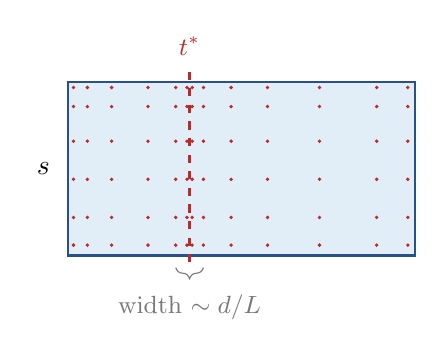
\begin{tikzpicture}[scale=2.2]
  \fill[cCell] (0,0) rectangle (2,1);
  \draw[cElem,thick] (0,0) rectangle (2,1);
  \node[left] at (-0.05,0.5) {$s$};
  \foreach \s in {0.06,0.22,0.44,0.66,0.86,0.97} {
    \foreach \t in {0.03,0.11,0.25,0.46,0.62,0.685,0.715,0.78,0.94,1.15,1.45,1.78,1.96} {
      \fill[cTrg] (\t,\s) circle (0.011);
    }
  }
  \draw[dashed,cTrg,thick] (0.70,-0.04) -- (0.70,1.10);
  \node[cTrg,above,font=\small] at (0.70,1.10) {$t^\ast$};
  \draw[decorate,decoration={brace,amplitude=4pt,mirror},cGrey] (0.62,-0.07) -- (0.78,-0.07);
  \node[cGrey,below,font=\small] at (0.70,-0.17) {width $\sim d/L$};
\end{tikzpicture}
\end{document}
